\documentclass{ijcaArticle}
\setcounter{page}{1}
\ijcaVolume{*}
\ijcaNumber{*}
\ijcaYear{2024}
\ijcaMonth{August}

\usepackage{amsmath,amssymb,amsfonts}
\usepackage{textcomp}
\usepackage{xcolor}
\usepackage{grffile}
\usepackage{graphicx}
\graphicspath{{figures/}{./}{Thesis/}}

\hyphenpenalty=5000
\exhyphenpenalty=5000
\sloppy

\begin{document}

\title{Comparative Performance and Computational Complexity Analysis of Pre-Trained Deep Learning Models for Citrus Fruit Disease Classification}

\author{ 
   \large Nur E Jannatul Farjana \\[-3pt]
   \normalsize Dept. of Computer Science and Engineering \\[-3pt]
   \normalsize International University of Business Agriculture and Technology \\[-3pt]
   \normalsize Uttara, Dhaka-1230, Bangladesh \\[-3pt]
  \and
   \large Abdullah Miraz \\[-3pt]
   \normalsize Dept. of Computer Science and Engineering \\[-3pt]
   \normalsize International University of Business Agriculture and Technology \\[-3pt]
   \normalsize Uttara, Dhaka-1230, Bangladesh \\[-3pt]
  \and
   \large Krishna Das \\[-3pt]
   \normalsize Dept. of Computer Science and Engineering \\[-3pt]
   \normalsize International University of Business Agriculture and Technology \\[-3pt]
   \normalsize Uttara, Dhaka-1230, Bangladesh \\[-3pt]
}

\terms{Algorithms, Experimentation, Performance}
\keywords{Transfer Learning, Convolutional Neural Networks, Citrus Disease Classification, Performance Metrics, Computational Complexity, MobileNetV2}

\maketitle

\begin{abstract} 
Early recognition of citrus fruit pathologies is critical for minimizing post-harvest economic losses and disease spread in commercial orchards. This paper evaluates the practical trade-offs between classification performance and hardware runtime costs across four pre-trained deep neural networks: MobileNetV2, InceptionV3, ResNet50, and VGG19. Models were trained and tested on 1,463 RGB images spanning four classes: citrus canker, black spot, Huanglongbing (greening), and healthy fruit. Experimental benchmarks indicate that MobileNetV2 attains the highest test classification rate (96.77\% overall accuracy and 98.54\% F1-score) while maintaining a compact memory footprint of 9.82~MB and a training time of 406.29~s. InceptionV3 performed similarly in accuracy (96.59\%) but with larger memory overhead (22.81~MB). ResNet50 underperformed under fixed-base fine-tuning (58.21\% F1-score), and VGG19 proved computationally heavy (3360.14~s training time, 118.59~MB footprint). Overall, depthwise separable architectures offer an effective operational profile for real-time mobile and edge-based field diagnosis.
\end{abstract}

\section{Introduction}

In Bangladesh, agriculture generates substantial rural employment and provides staple food security across the country. Commercial fruit farming, particularly citrus cultivation (limes, lemons, oranges, and grapefruits), has grown rapidly over the past five decades, expanding from 19,163 tonnes in 1973 to 175,325 tonnes in 2022 \cite{p22}. However, regional orchards in districts such as Sylhet, Moulvibazar, and Habiganj face persistent losses from bacterial and fungal pathogens, including citrus canker, black spot, scab, and Huanglongbing (greening) \cite{p5,p19}. When infections spread unchecked, fruit yield drops significantly, and cosmetic damage lowers market value \cite{p1,p2,p19}.

Traditional disease inspection relies on manual orchard scouting by agricultural extension officers or farmers. This process is labor-intensive, error-prone, and slow over large acreages \cite{p10,p21}. Computer vision systems offer an automated alternative by processing RGB images taken directly in the field \cite{p3,p20}. Convolutional neural networks (CNNs), in particular, have shown strong capability in learning discriminative visual features from plant leaf and fruit images \cite{p5}. Canonical architectures such as AlexNet, VGG16, VGG19, InceptionV3, ResNet, and DenseNet have established high efficacy on botanical image datasets.

\subsection{Context and Background}

Across rural Bangladesh, smallholder farmers depend heavily on seasonal fruit harvests for household income \cite{p6,p8}. More than 39,678 acres of land are currently allocated to fruit and crop production nationwide \cite{p7,p6}. Because field environments are vulnerable to sudden microclimatic shifts and pest-borne infections, timely diagnosis is essential to guide targeted spraying \cite{p19,p20}. Automated screening reduces both broad-spectrum pesticide waste and operational labor costs.

\subsection{Research Motivation}

Several recent publications have demonstrated high accuracy using deep CNNs for plant disease detection \cite{p2, p5, p8}. However, many of these studies rely on heavyweight networks (e.g., AlexNet or VGG19) that demand high computational throughput, large GPU allocations, and lengthy training cycles \cite{p5}. In real agricultural settings, diagnostic software must often run locally on smartphones, microcontroller modules, or camera-equipped drones with constrained battery life and memory. Few existing studies measure the practical run-time latency, storage footprint, or memory consumption of their models alongside raw accuracy. This paper addresses that gap by testing both diagnostic metrics and computational overhead across four pre-trained networks.

\subsection{Objectives and Scope}
The investigation focuses on three specific goals:
\begin{itemize}
    \item Fine-tuning four pre-trained CNN models (MobileNetV2, InceptionV3, ResNet50, and VGG19) using transfer learning on 1,463 citrus fruit images across four distinct conditions.
    \item Measuring classification metrics (accuracy, precision, recall, F1-score) and hardware-oriented parameters (training time, test inference latency, parameter count, RAM usage).
    \item Identifying the most viable model architecture for deployment on portable, battery-powered agricultural hardware.
\end{itemize}

\subsection{Significance of Research}
This work provides empirical benchmarks linking diagnostic accuracy directly to embedded hardware constraints in citrus disease detection. The data provides concrete engineering reference points for building field-ready mobile apps and drone scouting systems.

The subsequent sections cover related literature (Section~\ref{sec:literature_review}), experimental methodology and model configurations (Section~\ref{sec:proposed_methodology}), performance evaluation and complexity benchmarks (Section~\ref{sec:result_and_discussion}), and conclusions with future directions (Section~\ref{sec:conclusion}).

\section{Literature Review}
\label{sec:literature_review}

Agricultural activities support nearly 87\% of the rural population in Bangladesh through direct cultivation and local markets \cite{p9}. For this reason, automated image screening for early disease detection has drawn substantial research interest.

Ahmed and Muqit \cite{p2} built a deep neural network pipeline for citrus fruit and leaf infection screening across a 2,293-image PlantVillage subset, reaching 94.55\% accuracy. Balafas et al. \cite{p3} compared traditional machine learning models (Support Vector Machines, Random Forests, SGD) against deeper networks (InceptionV3, VGG16, VGG19), showing that deep features handle background noise and field illumination changes more reliably than shallow hand-crafted descriptors.

\begin{table*}[t]
\tabcolsep4pt
\tbl{Summary of Related Literature on Citrus and Plant Disease Detection}{
\begin{tabular}{|c|l|c|p{4.2cm}|p{2.8cm}|p{3.8cm}|c|}
\hline
\textbf{No.} & \textbf{Author} & \textbf{Year} &
\textbf{Class Types} & \textbf{Dataset Size} & \textbf{Classifier Architecture} &
\textbf{Accuracy} \\
\hline
1 & R. Sujatha et al. \cite{p10} & 2021 &
Black spot, Canker, Greening, Melanose, Healthy &
609 images &
LSVM, SGD, RF, InceptionV3, VGG16, VGG19 &
89.5\% \\
\hline
2 & Khattak et al. \cite{p7} & 2021 &
Black spot, Canker, Scab, Greening, Melanose, Healthy &
2293 (Fruits+Leaves) &
Custom CNN + Softmax &
94.55\% \\
\hline
3 & A. Elaraby et al. \cite{p5} & 2022 &
Anthracnose, Black spot, Canker, Scab, Greening, Melanose &
759 (Fruits+Leaves) &
AlexNet, VGG19 &
94.0\% \\
\hline
4 & S. Parez et al. \cite{p18} & 2023 &
Multiple plant pathological conditions &
Plant leaves &
Lightweight CNN + Softmax &
99.0\% \\
\hline
5 & Dehuan Luo et al. \cite{p11} & 2023 &
Anthracnose, Canker, Melanosis, Scab, Brown Spot, Leaf Miner &
3202 images &
Light-SA YOLOv8 &
92.6\% \\
\hline
6 & Madhusudan G. et al. \cite{p17} & 2023 &
Black spot, Melanose, Canker, Greening, Healthy &
609 RGB images &
CNN, ResNet152V2, DenseNet121, InceptionResNetV2 &
98.0\% \\
\hline
7 & Poonam Dhiman et al. \cite{p12} & 2023 &
HLB, Black spot, Melanose, Canker, Scab &
2950 images &
CNN + LSTM &
98.25\% \\
\hline
8 & W. G{\'o}mez-Flores et al. \cite{p13} & 2024 &
HLB, Greasy spot, Deficiencies, Citrus Mite, Red scale &
953 images &
DNN, Transfer Learning &
Not reported \\
\hline
9 & Nouman Butt et al. \cite{p14} & 2024 &
Canker, Citrus scab, Black spot &
2184 images &
SVM, KNN &
99.6\% \\
\hline
10 & J. Shermila et al. \cite{p15} & 2024 &
Fruit blight, Greening, Scab, Melanoses &
759 images &
Custom CNN + LSTM &
96.0\% \\
\hline
11 & A.K. Saini et al. \cite{p16} & 2024 &
Anthracnose, Melanose, Brown Spot &
759 images &
SADCNN-ORBM &
99.76\% \\
\hline
\end{tabular}}
\label{tab:citrus_comparison}
\end{table*}

Elaraby et al. \cite{p5} achieved 94.0\% accuracy classifying multiple citrus conditions using AlexNet and VGG19 backbones. Sujatha et al. \cite{p10} evaluated deep architectures for mobile plant pathology tools, emphasizing the need for accessible field-level diagnostics. Hasan et al. \cite{p6,p24} utilized transfer learning on regional crop datasets in Bangladesh, noting that pre-trained weights from ImageNet significantly improve feature convergence on small target datasets. Table~\ref{tab:citrus_comparison} summarizes recent related studies in citrus and general plant disease detection.

\section{Proposed Methodology}
\label{sec:proposed_methodology}

The experimental pipeline spans data acquisition, class-balanced partitioning, real-time image augmentation, transfer learning model adaptation, Adam optimization, and metric evaluation. Figure~\ref{fig:research design} illustrates the complete workflow.

\begin{figure}[t]
    \centerline{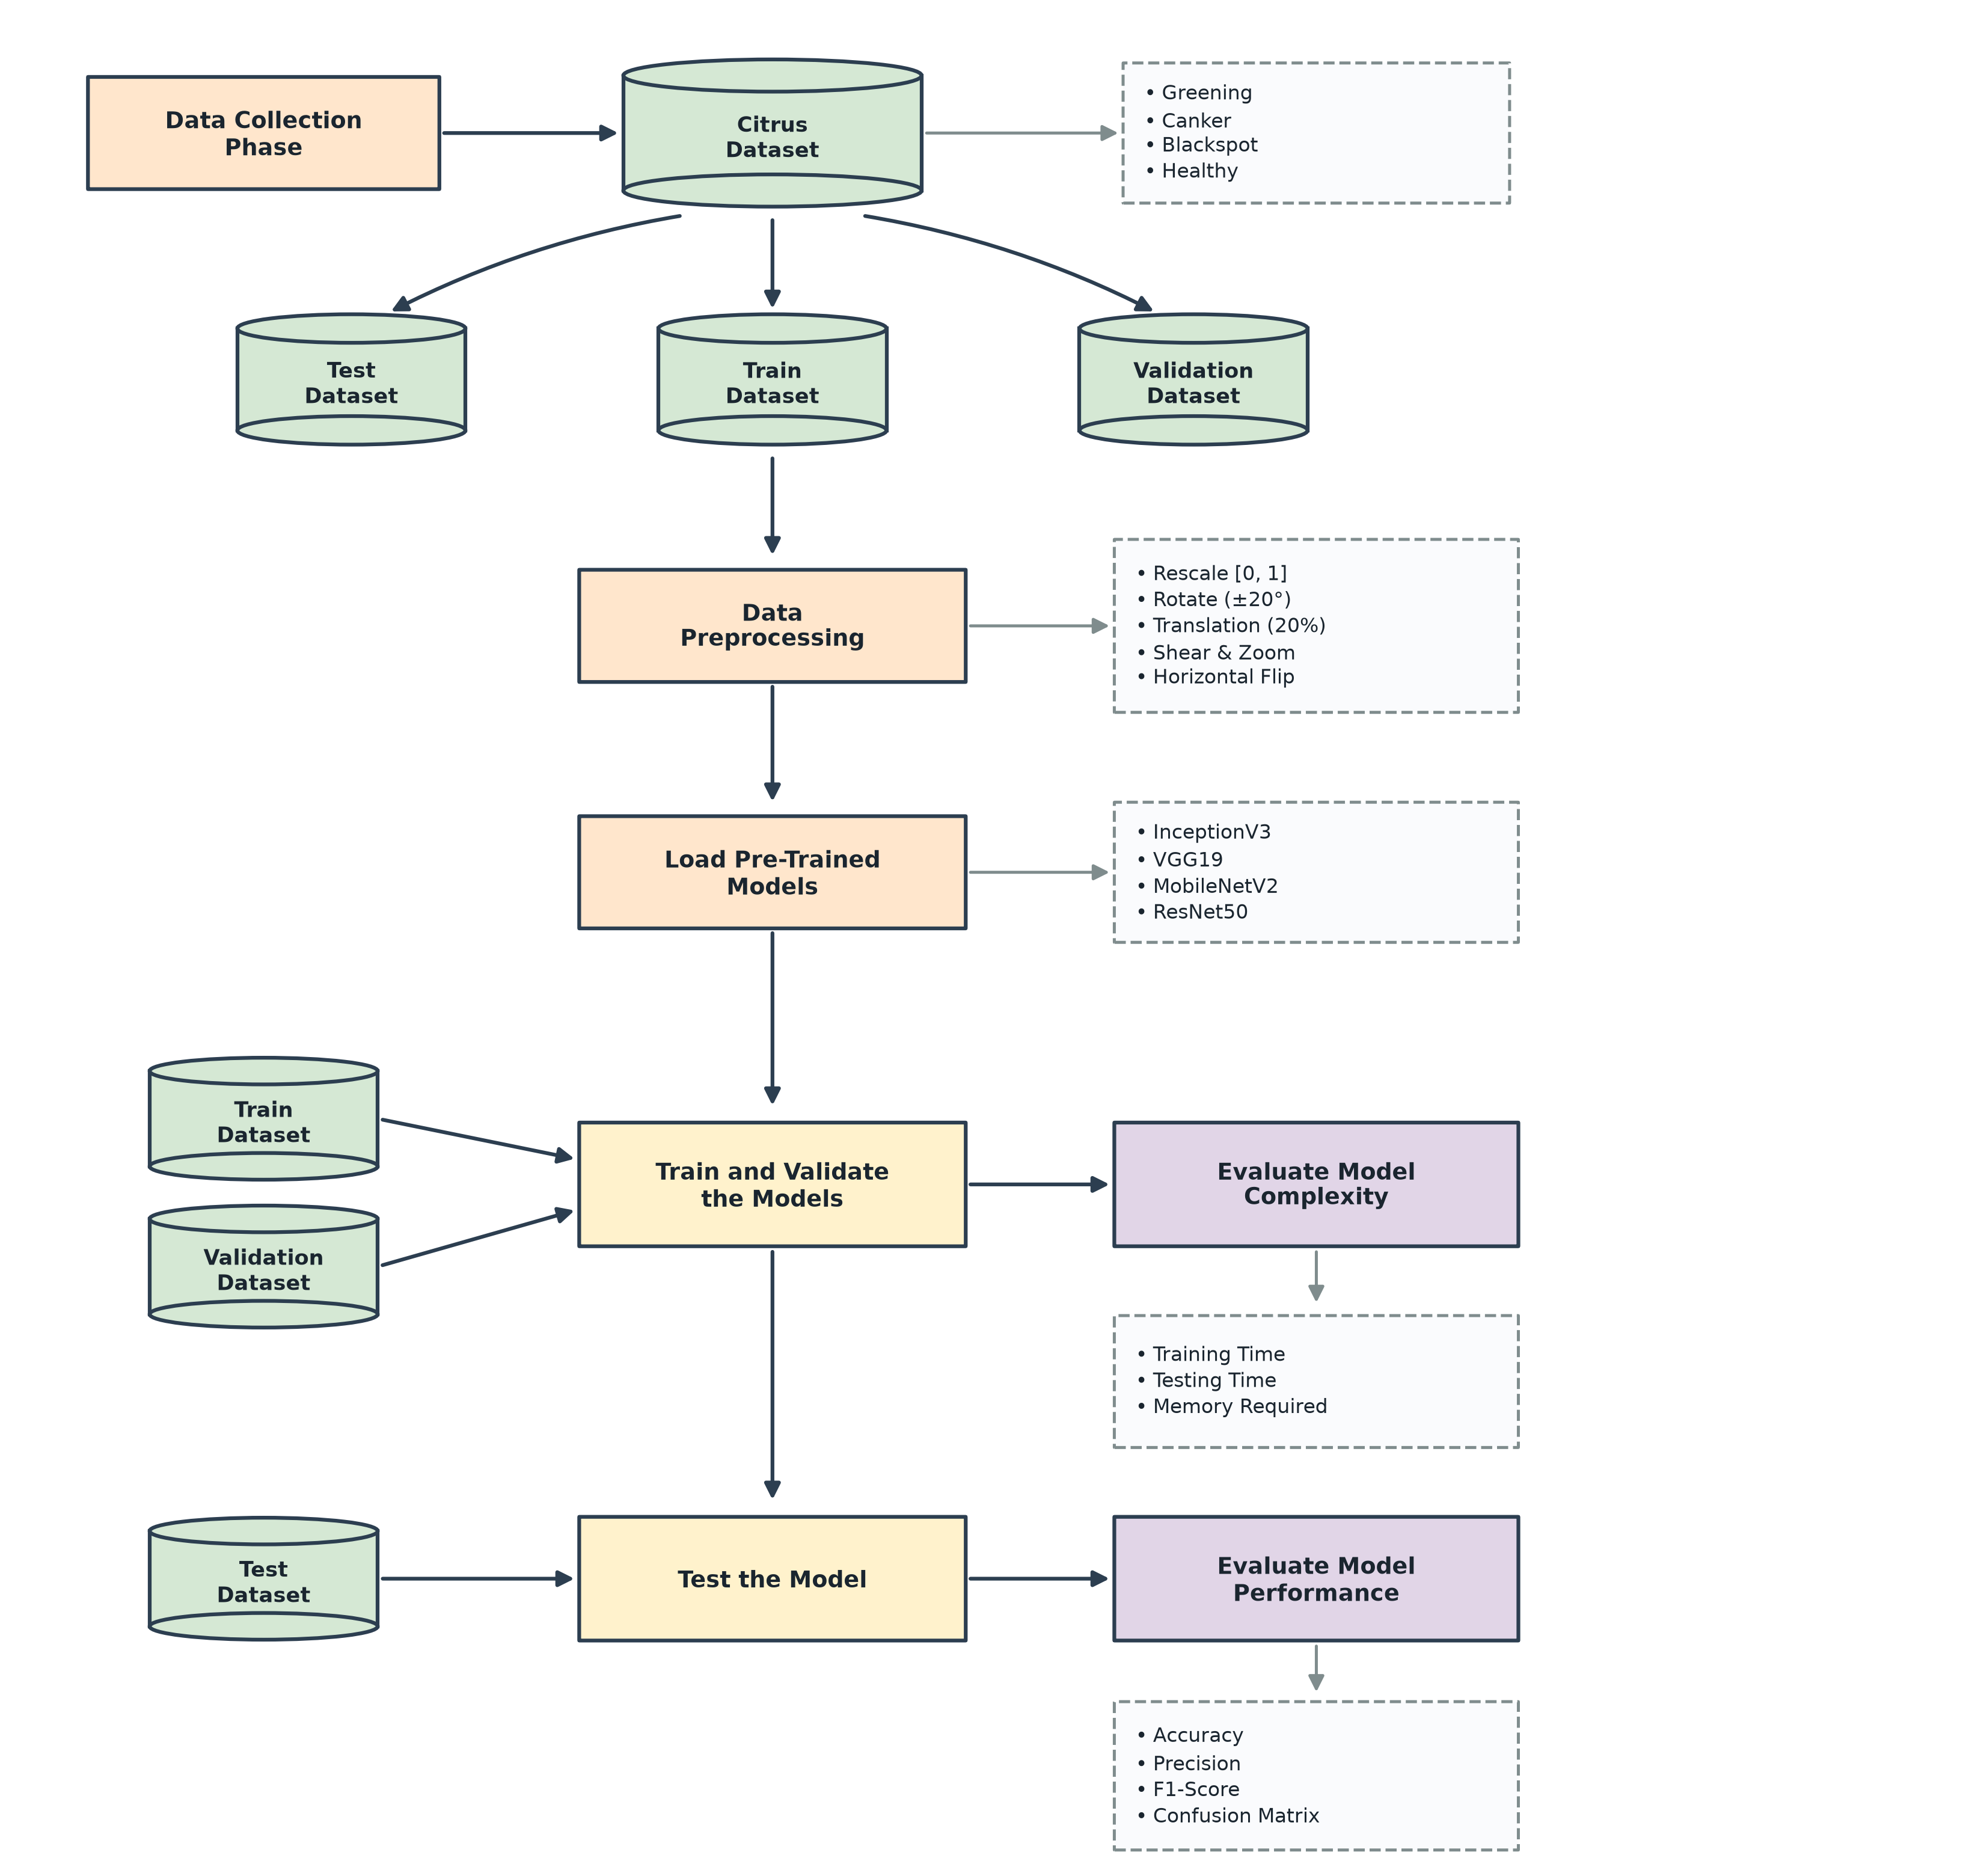
\includegraphics[width=0.88\columnwidth]{fig1_methodology.png}}
    \caption{End-to-end methodological framework for citrus fruit disease classification.}
    \label{fig:research design}
\end{figure}

\subsection{Dataset Overview and Preparation}
The experimental image corpus includes 1,463 high-resolution RGB samples obtained from PlantVillage and Kaggle repositories. The images are grouped into four primary classes:
\begin{itemize}
    \item \textbf{Canker}: Raised, rough lesions caused by the bacterial pathogen \textit{Xanthomonas citri}.
    \item \textbf{Black Spot}: Dark, circular necrotic spots caused by the fungus \textit{Phyllosticta citricarpa}.
    \item \textbf{Greening (HLB)}: Asymmetric fruit and foliage yellowing caused by vector-borne \textit{Candidatus} Liberibacter bacteria.
    \item \textbf{Healthy}: Uninfected fruit samples showing standard skin texture and coloration.
\end{itemize}

\subsubsection{Class Distribution and Partitioning}
Image files were indexed by class into structured metadata tables. As shown in Figure~\ref{fig:class}, the sample counts are well-balanced across categories: 358 healthy, 387 greening, 362 black spot, and 356 canker samples. Figure~\ref{fig:sample images} displays sample images from each class.

\begin{figure}[t]
    \centerline{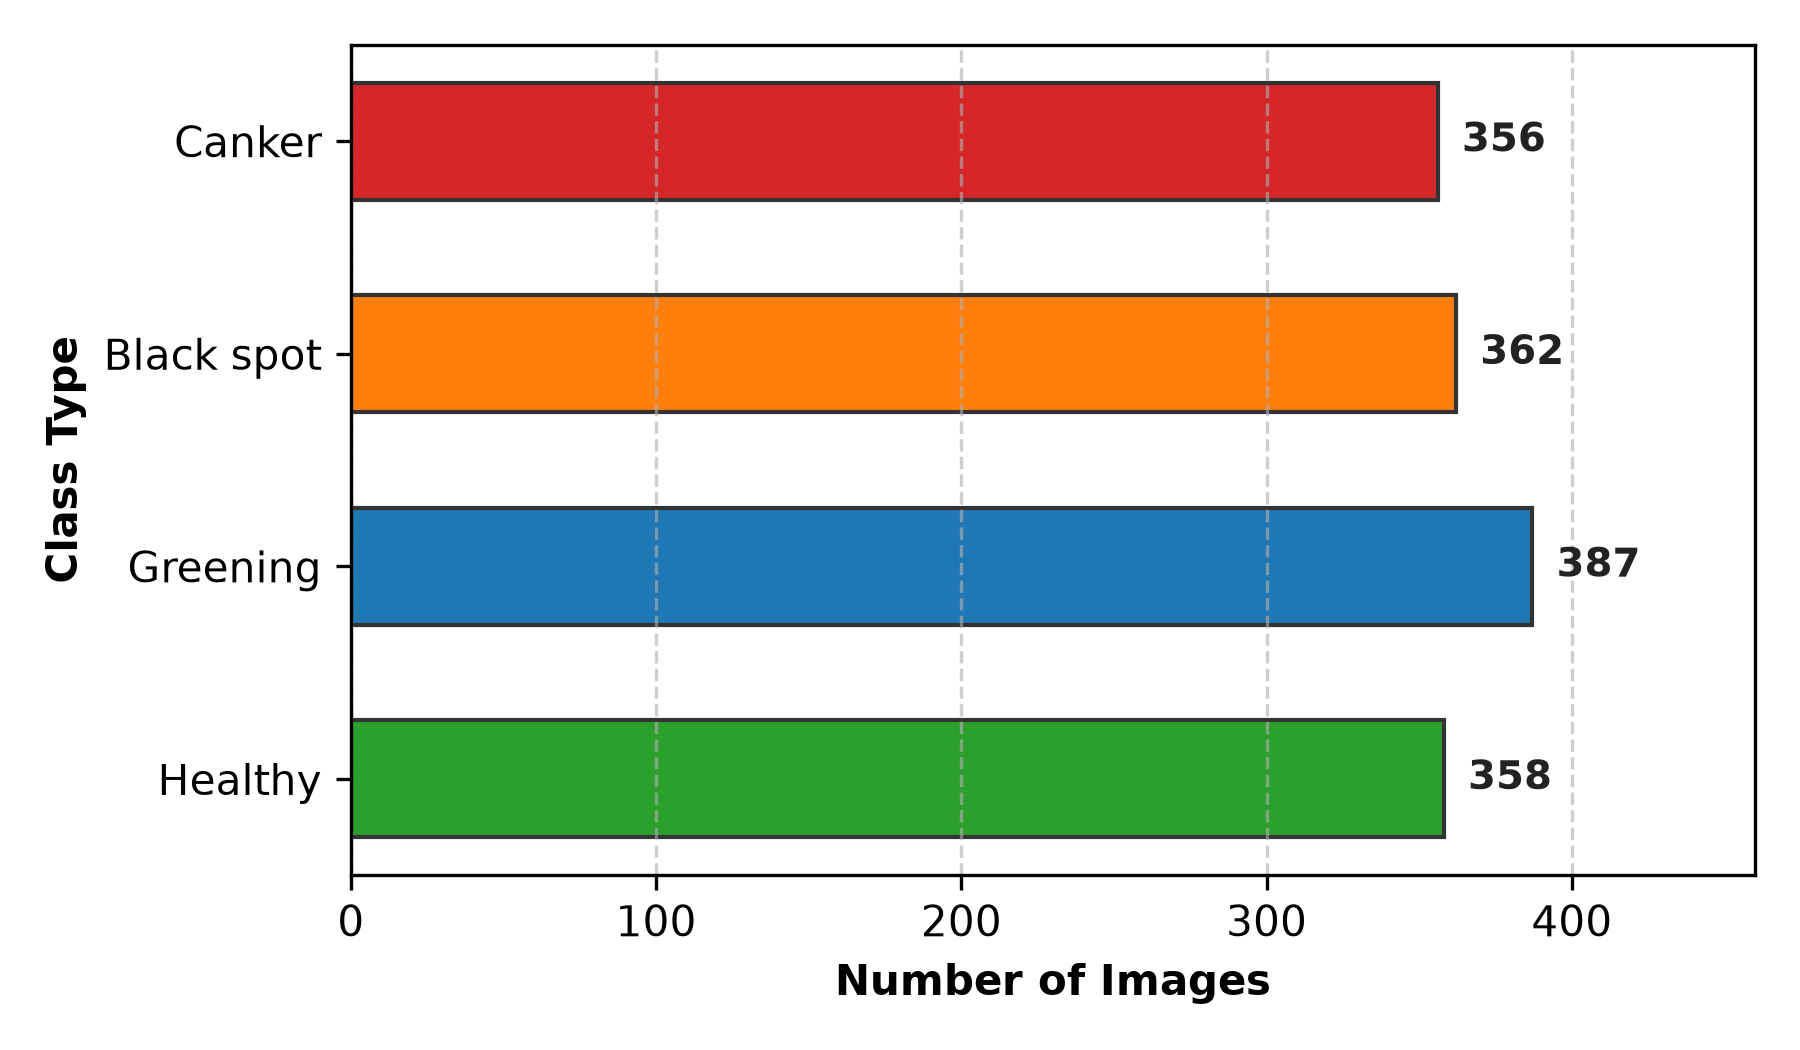
\includegraphics[width=0.88\columnwidth]{fig2_class_distribution.png}}
    \caption{Distribution of image samples across the four citrus fruit classes.}
    \label{fig:class}
\end{figure}

\begin{figure}[t]
    \centerline{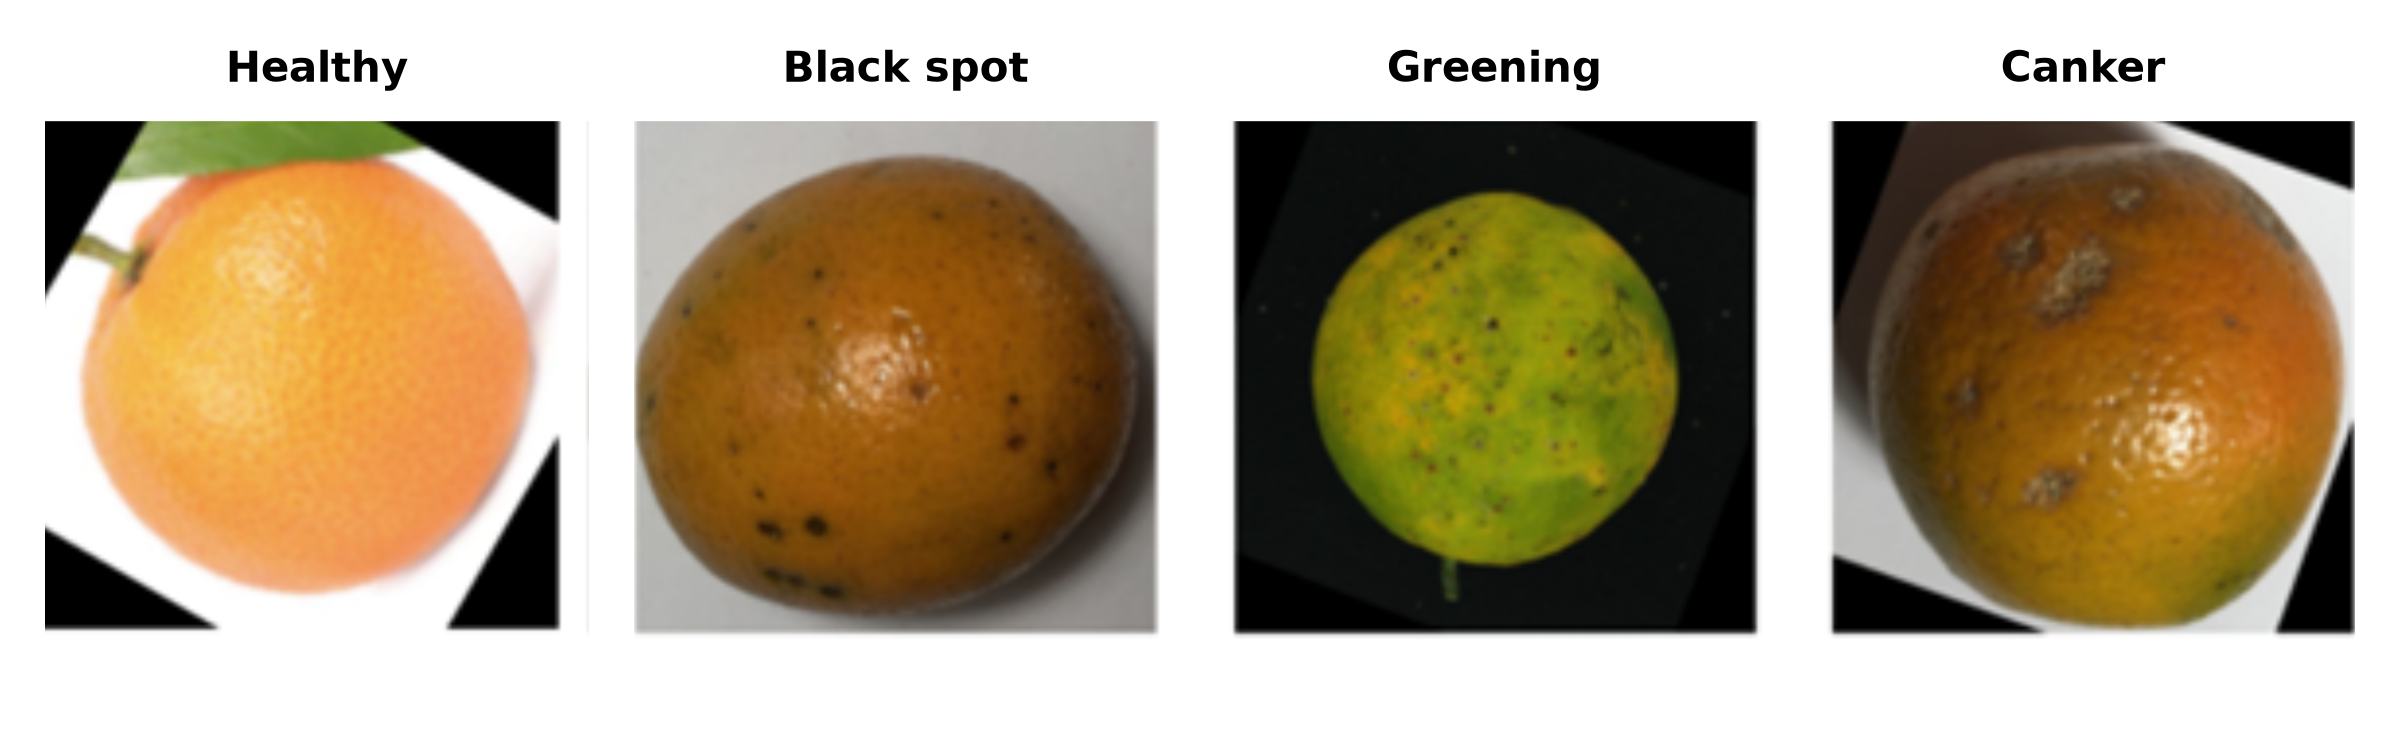
\includegraphics[width=0.88\columnwidth]{fig3_sample_images.png}}
    \caption{Representative sample images from the experimental citrus dataset.}
    \label{fig:sample images}
\end{figure}

The dataset was divided into an 80\% training split (1,170 images), a 10\% validation split (146 images), and a 10\% test split (147 images), illustrated in Figure~\ref{fig:dataset split}. The test split was isolated and evaluated only after training was fully completed.

\begin{figure}[t]
    \centerline{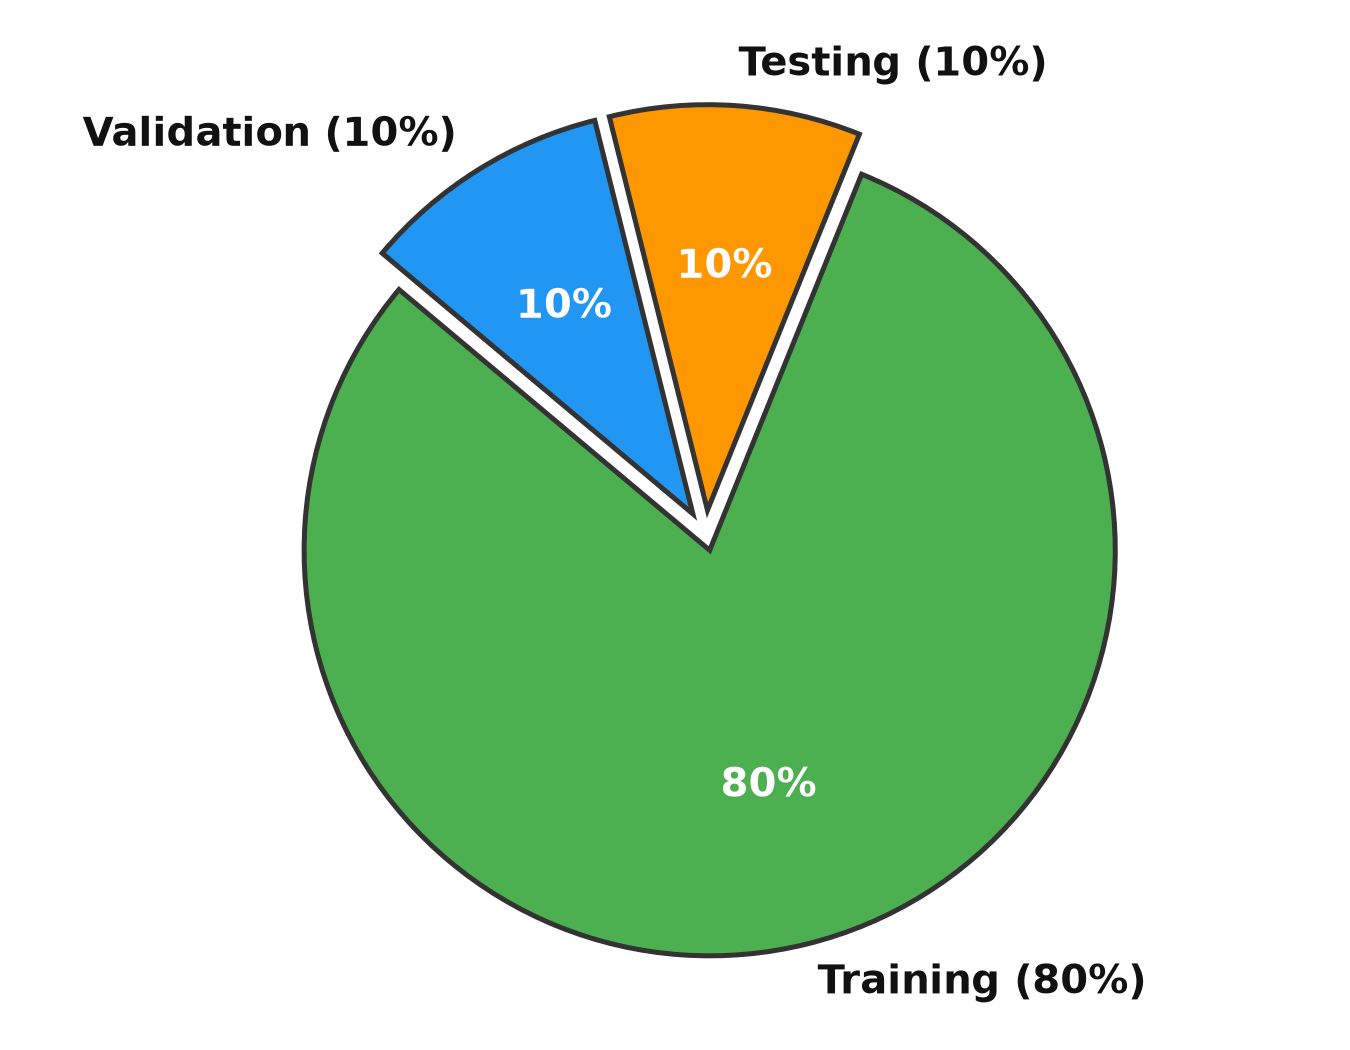
\includegraphics[width=0.72\columnwidth]{fig4_dataset_split.png}}
    \caption{Dataset partitioning into training (80\%), validation (10\%), and test (10\%) subsets.}
    \label{fig:dataset split}
\end{figure}

\subsubsection{Data Pre-Processing and Augmentation}
To reduce overfitting and improve model invariance to field camera angles and lighting, real-time data augmentations were applied to the training pipeline:
\begin{itemize}
    \item Intensity normalization scaling pixel values to $[0, 1]$.
    \item Random rotations up to $\pm 20^\circ$.
    \item Horizontal and vertical translations up to 20\%.
    \item Random shear mappings.
    \item Random zoom scaling up to 20\%.
    \item Random horizontal reflections.
\end{itemize}
All images were resized to standard dimensions of $224 \times 224 \times 3$ pixels and grouped into mini-batches of 32 samples.

\subsection{Transfer Learning Framework}

Transfer learning leverages representational weights pre-trained on large datasets (such as ImageNet) to extract features efficiently on smaller specialized agricultural sets \cite{p25,p24}. Figure~\ref{fig:pretrained} shows the adaptation process.

\begin{figure}[t]
    \centerline{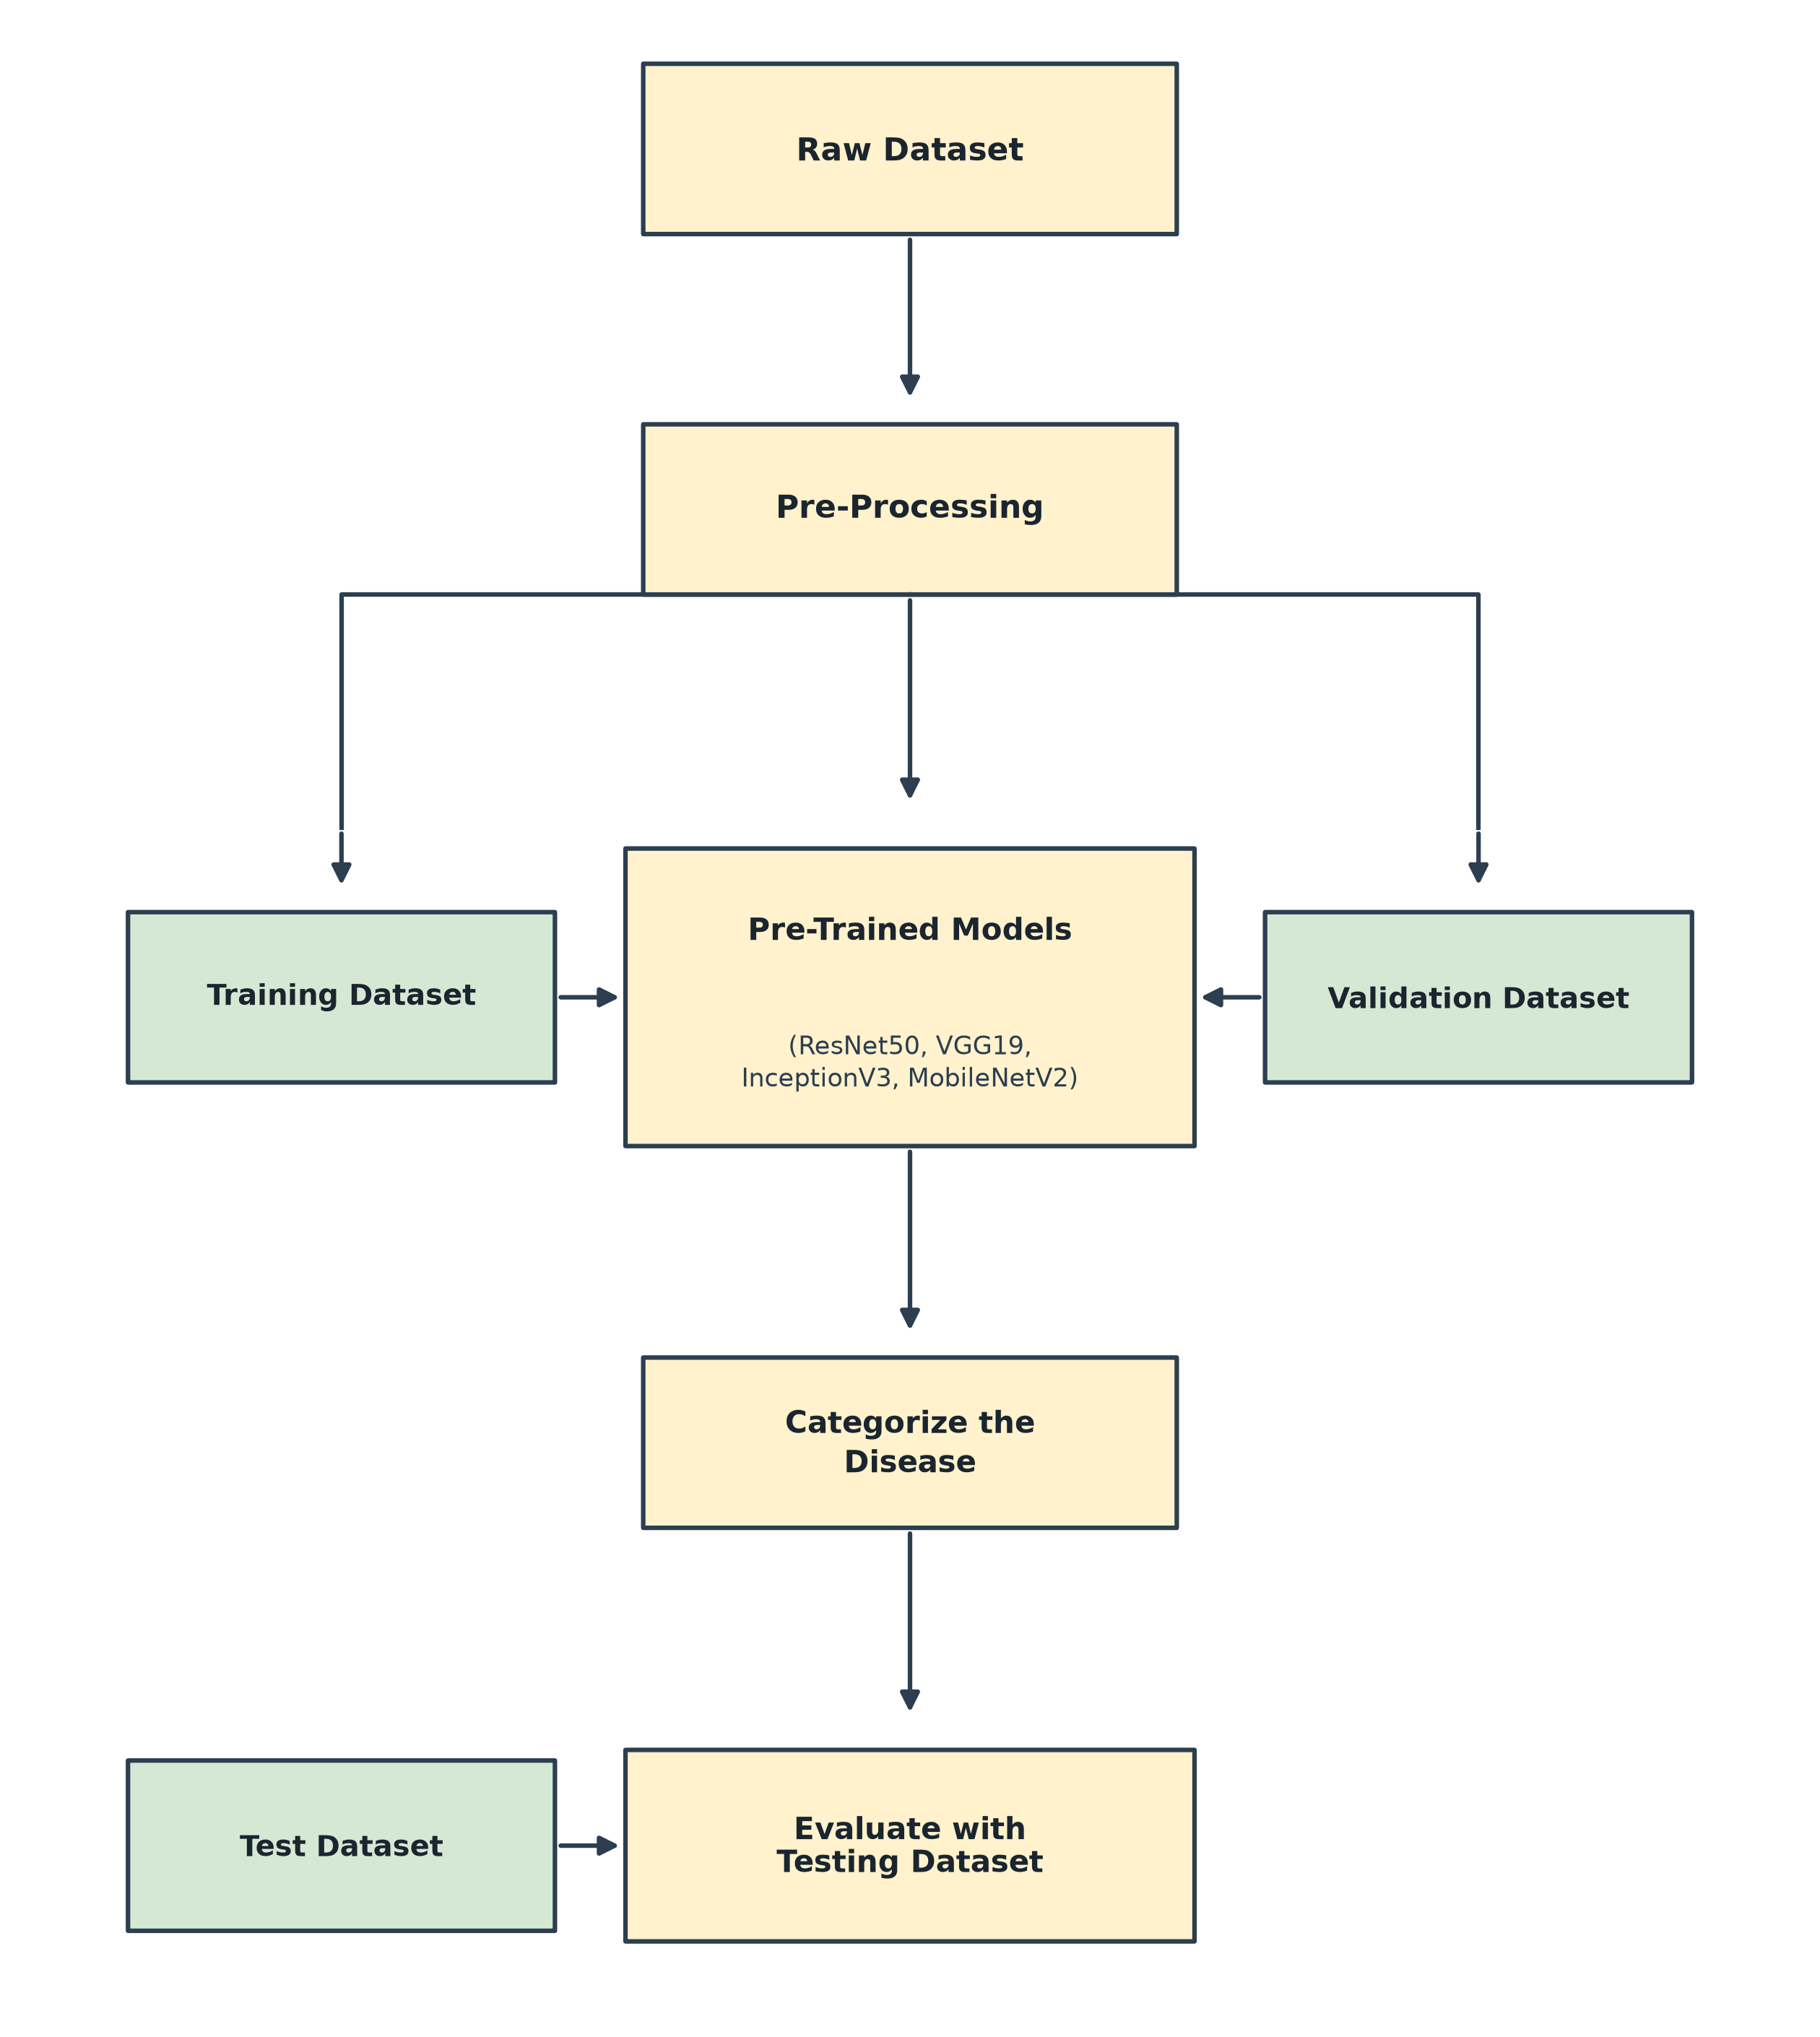
\includegraphics[width=0.72\columnwidth]{fig5_pretrained_workflow.png}}
    \caption{Flowchart of the transfer learning fine-tuning pipeline.}
    \label{fig:pretrained}
\end{figure}

Four CNN architectures were tested with identical classifier heads:
\begin{itemize}
    \item \textbf{VGG19}: Built with 16 convolutional layers and 3 dense layers using uniform $3 \times 3$ filters \cite{p38,p39,p40}. The convolutional base was frozen during training. The custom classification head includes a 40\% Dropout layer \cite{p41,p42,p43}, a Flatten layer \cite{p44}, a Dense layer with 512 ReLU units, a 20\% Dropout layer, and a 4-unit Softmax output layer \cite{p45}. Table~\ref{tab:model_architecture} lists the layer details.

\begin{table}[htbp]
\tabcolsep4pt
\tbl{Layer Architecture and Parameter Details of Fine-Tuned VGG19}{
\begin{tabular}{|l|c|r|}
\hline
\textbf{Layer (Type)} & \textbf{Output Shape} & \textbf{Parameters} \\
\hline
VGG19 (Functional Base) & (None, 7, 7, 512) & 20,024,384 \\
dropout\_1 (Dropout 40\%) & (None, 7, 7, 512) & 0 \\
flatten (Flatten) & (None, 25088) & 0 \\
dense\_1 (Dense, ReLU) & (None, 512) & 12,845,056 \\
dropout\_2 (Dropout 20\%) & (None, 512) & 0 \\
dense\_2 (Dense, Softmax) & (None, 4) & 2,052 \\
\hline
\multicolumn{2}{|l|}{\textbf{Total Parameters:}} & 32,871,492 \\
\multicolumn{2}{|l|}{\textbf{Trainable Parameters:}} & 12,847,108 \\
\multicolumn{2}{|l|}{\textbf{Non-Trainable Parameters:}} & 20,024,384 \\
\hline
\end{tabular}}
\label{tab:model_architecture}
\end{table}

    \item \textbf{MobileNetV2}: Employs depthwise separable convolutions and inverted residual bottlenecks with linear activation units \cite{p37}. The base weights were kept frozen, followed by the same top dense layers. Table~\ref{tab:mobilenetv2} outlines the layer layout.

\begin{table}[htbp]
\tabcolsep4pt
\tbl{Layer Architecture and Parameter Details of Fine-Tuned MobileNetV2}{
\begin{tabular}{|l|c|r|}
\hline
\textbf{Layer (Type)} & \textbf{Output Shape} & \textbf{Parameters} \\
\hline
MobileNetV2 (Base) & (None, 7, 7, 1280) & 2,257,984 \\
dropout\_1 (Dropout 40\%) & (None, 7, 7, 1280) & 0 \\
flatten (Flatten) & (None, 62720) & 0 \\
dense\_1 (Dense, ReLU) & (None, 512) & 32,085,760 \\
dropout\_2 (Dropout 20\%) & (None, 512) & 0 \\
dense\_2 (Dense, Softmax) & (None, 4) & 2,052 \\
\hline
\multicolumn{2}{|l|}{\textbf{Total Parameters:}} & 34,345,796 \\
\multicolumn{2}{|l|}{\textbf{Trainable Parameters:}} & 32,087,812 \\
\multicolumn{2}{|l|}{\textbf{Non-Trainable Parameters:}} & 2,257,984 \\
\hline
\end{tabular}}
\label{tab:mobilenetv2}
\end{table}

    \item \textbf{InceptionV3}: Incorporates multi-scale inception modules with factorized asymmetric convolutions. A custom top head with Flatten, 512-unit Dense ReLU, Dropout (20\%), and 4-unit Softmax was appended. Table~\ref{tab:inceptionv3} presents the layer summary.

\begin{table}[htbp]
\tabcolsep4pt
\tbl{Layer Architecture and Parameter Details of Fine-Tuned InceptionV3}{
\begin{tabular}{|l|c|r|}
\hline
\textbf{Layer (Type)} & \textbf{Output Shape} & \textbf{Parameters} \\
\hline
InceptionV3 (Base) & (None, 5, 5, 2048) & 21,802,784 \\
flatten (Flatten) & (None, 51200) & 0 \\
dense\_1 (Dense, ReLU) & (None, 512) & 26,214,912 \\
dropout\_2 (Dropout 20\%) & (None, 512) & 0 \\
dense\_2 (Dense, Softmax) & (None, 4) & 2,052 \\
\hline
\multicolumn{2}{|l|}{\textbf{Total Parameters:}} & 48,019,748 \\
\multicolumn{2}{|l|}{\textbf{Trainable Parameters:}} & 26,216,964 \\
\multicolumn{2}{|l|}{\textbf{Non-Trainable Parameters:}} & 21,802,784 \\
\hline
\end{tabular}}
\label{tab:inceptionv3}
\end{table}

    \item \textbf{ResNet50}: Uses residual shortcut connections to pass gradients directly across deep residual blocks. The top pooling was replaced with Flatten, Dense (512 units), 50\% Dropout, and 4-class Softmax. Table~\ref{tab:resnet50} provides the layer parameters.

\begin{table}[htbp]
\tabcolsep4pt
\tbl{Layer Architecture and Parameter Details of Fine-Tuned ResNet50}{
\begin{tabular}{|l|c|r|}
\hline
\textbf{Layer (Type)} & \textbf{Output Shape} & \textbf{Parameters} \\
\hline
ResNet50 (Base) & (None, 5, 5, 2048) & 23,587,712 \\
flatten (Flatten) & (None, 100352) & 0 \\
dense\_1 (Dense, ReLU) & (None, 512) & 51,380,736 \\
dropout\_2 (Dropout 50\%) & (None, 512) & 0 \\
dense\_2 (Dense, Softmax) & (None, 4) & 2,052 \\
\hline
\multicolumn{2}{|l|}{\textbf{Total Parameters:}} & 74,970,500 \\
\multicolumn{2}{|l|}{\textbf{Trainable Parameters:}} & 51,382,788 \\
\multicolumn{2}{|l|}{\textbf{Non-Trainable Parameters:}} & 23,587,712 \\
\hline
\end{tabular}}
\label{tab:resnet50}
\end{table}

\end{itemize}

\subsubsection{Framework Implementation}
All experiments were developed in Python using TensorFlow and Keras. The end-to-end framework, spanning data ingestion, GPU model training, model checkpointing, and mobile deployment export (TensorFlow Lite, TensorFlow Serving), is shown in Figure~\ref{fig:tensorflow}.

\begin{figure}[t]
    \centerline{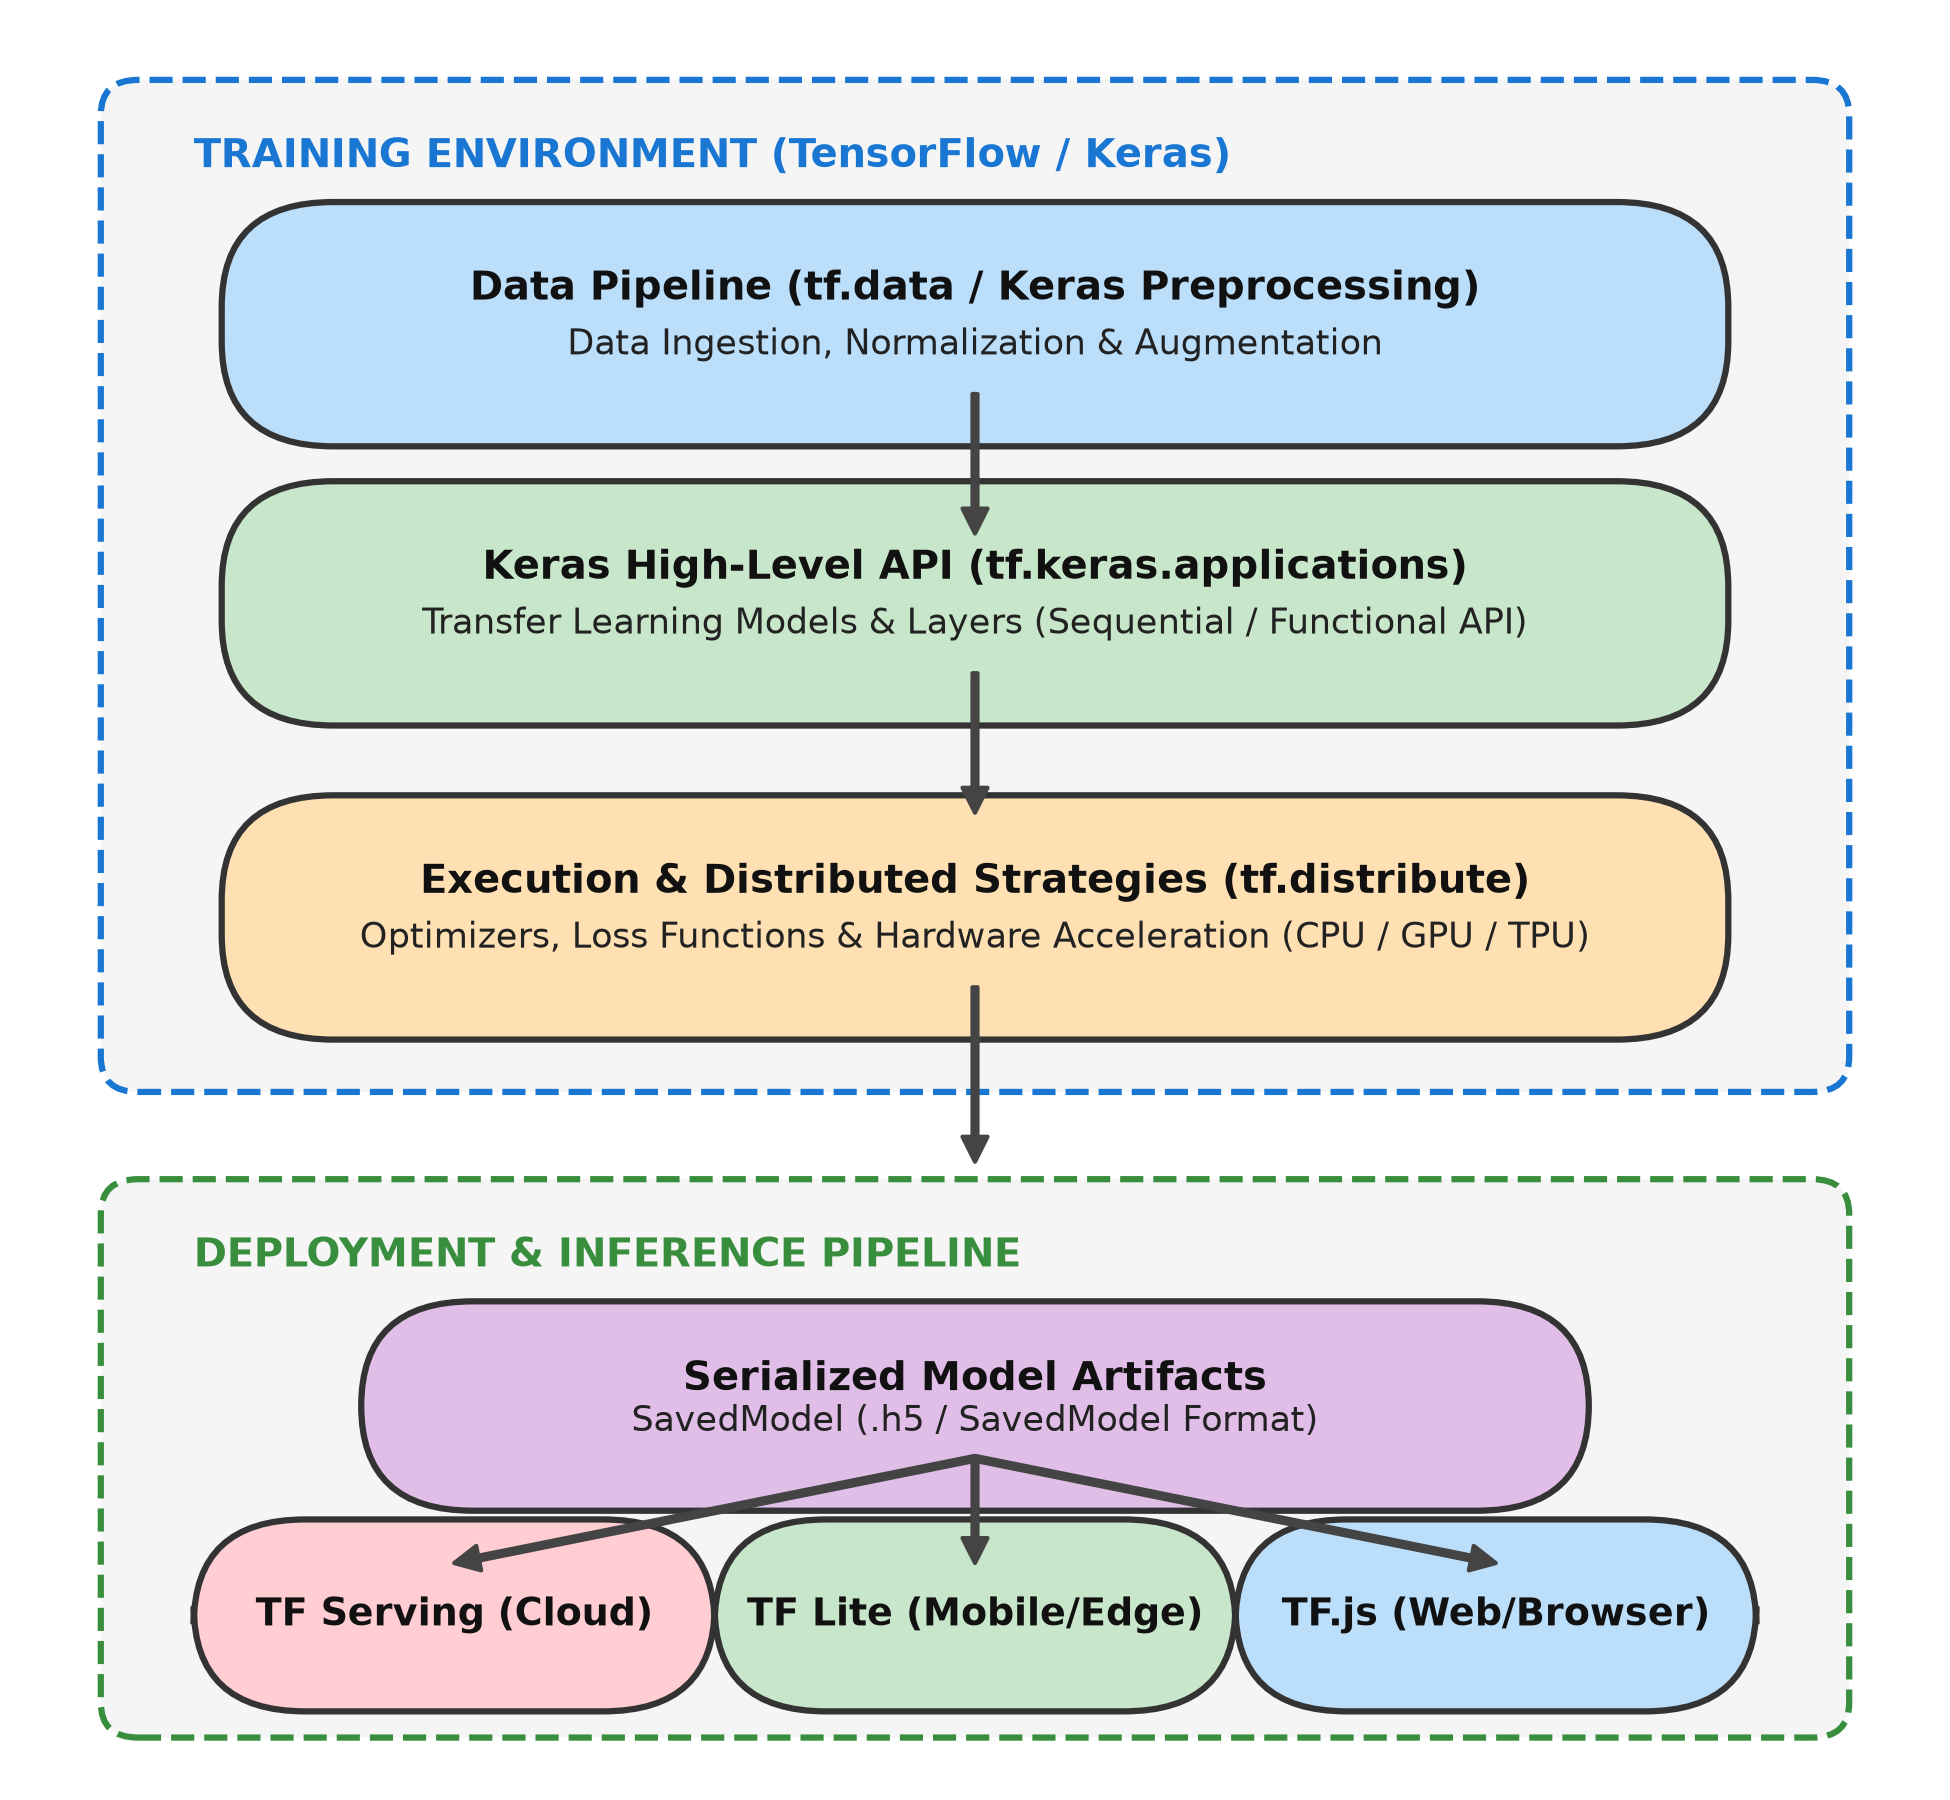
\includegraphics[width=0.88\columnwidth]{fig6_tensorflow_architecture.png}}
    \caption{Framework architecture covering training, serialization, and deployment pipelines.}
    \label{fig:tensorflow}
\end{figure}

\subsection{Optimization and Training Configuration}
All four architectures were trained with the Adam optimizer at a fixed learning rate of $\eta = 0.0001$. Categorical cross-entropy was applied as the training loss:
\begin{equation}
    \mathcal{L}_{CCE} = -\sum_{i=1}^{N} \sum_{c=1}^{C} y_{i,c} \log(\hat{y}_{i,c})
\end{equation}
where $N$ is the mini-batch size, $C=4$ is the number of target classes, $y_{i,c} \in \{0, 1\}$ is the true label, and $\hat{y}_{i,c}$ is the model predicted probability for class $c$. Training ran for 50 epochs with checkpointing monitoring validation loss.

\subsection{Evaluation Metrics}

\subsubsection{Diagnostic Performance Metrics}
Classification performance was measured using four standard indicators:
\begin{equation}
    \text{Accuracy} = \frac{TP + TN}{TP + TN + FP + FN}
    \label{eq:accuracy}
\end{equation}
\begin{equation}
    \text{Precision} = \frac{TP}{TP + FP}
    \label{eq:precision}
\end{equation}
\begin{equation}
    \text{Recall} = \frac{TP}{TP + FN}
    \label{eq:recall}
\end{equation}
\begin{equation}
    F1\text{-Score} = \frac{2 \cdot \text{Precision} \cdot \text{Recall}}{\text{Precision} + \text{Recall}}
    \label{eq:f1score}
\end{equation}
where $TP$, $TN$, $FP$, and $FN$ represent True Positives, True Negatives, False Positives, and False Negatives, respectively.

\subsubsection{Computational Complexity Metrics}
Hardware feasibility was evaluated across four operational parameters: total training wall-clock time (seconds), inference latency on the 147 test images (seconds), trainable/non-trainable parameter count, and dynamic memory consumption (MB).

\section{Result and Discussion}
\label{sec:result_and_discussion}

This section compares diagnostic accuracy and hardware runtime profiles across the four evaluated networks.

\subsection{Diagnostic Performance Evaluation}

Table~\ref{tab:performance_metrics} summarizes precision, recall, and F1-score for each model on the 147-image test partition. MobileNetV2 achieved the strongest overall performance, recording 98.56\% precision, 98.54\% recall, and 98.54\% F1-score. InceptionV3 followed closely, attaining 97.21\% precision, 97.30\% recall, and 97.19\% F1-score. VGG19 reached 84.82\% precision and 81.17\% F1-score. ResNet50 showed lower performance under this fine-tuning regime, yielding an F1-score of 58.21\%.

\begin{table}[htbp]
\tabcolsep4pt
\tbl{Performance Comparison Across Fine-Tuned Models on the Unseen Test Set}{
\begin{tabular}{|l|c|c|c|c|}
\hline
\textbf{Model Name} & \textbf{MobileNetV2} & \textbf{InceptionV3} & \textbf{ResNet50} & \textbf{VGG19} \\
\hline
Precision (\%) & 98.56 & 97.21 & 66.66 & 84.82 \\
Recall (\%) & 98.54 & 97.30 & 62.02 & 81.31 \\
F1-Score (\%) & 98.54 & 97.19 & 58.21 & 81.17 \\
\hline
\end{tabular}}
\label{tab:performance_metrics}
\end{table}

\subsubsection{Accuracy and Loss Trajectory Analysis}
Table~\ref{tab:evaluation_accuracy_loss} details training, validation, and test accuracies along with loss values for all four models. MobileNetV2 attained 97.29\% test accuracy with a low test loss of 5.29\%. InceptionV3 reached 96.59\% test accuracy (7.44\% loss). VGG19 achieved 88.44\% test accuracy with 37.76\% loss. ResNet50 recorded a test accuracy of 67.34\% with a higher loss of 76.16\%, indicating that residual blocks may need deeper layer unfreezing or adapted learning rates to transfer well to this dataset.

\begin{table}[htbp]
\tabcolsep2.5pt
\tbl{Accuracy and Loss Metrics Across Training, Validation, and Test Phases}{
\begin{tabular}{|l|c|c|c|c|c|c|}
\hline
\textbf{Model} & \multicolumn{2}{c|}{\textbf{Training}} &
\multicolumn{2}{c|}{\textbf{Validation}} &
\multicolumn{2}{c|}{\textbf{Testing}} \\
\hline
& \textbf{Acc. (\%)} & \textbf{Loss (\%)} &
\textbf{Acc. (\%)} & \textbf{Loss (\%)} &
\textbf{Acc. (\%)} & \textbf{Loss (\%)} \\
\hline
MobileNetV2 & 95.80 & 10.97 & 94.55 & 12.80 & 97.29 & 5.29 \\
InceptionV3 & 95.89 & 10.60 & 97.95 & 6.72 & 96.59 & 7.44 \\
ResNet50   & 57.14 & 96.91 & 61.90 & 83.92 & 67.34 & 76.16 \\
VGG19      & 75.10 & 60.10 & 87.75 & 32.46 & 88.44 & 37.76 \\
\hline
\end{tabular}}
\label{tab:evaluation_accuracy_loss}
\end{table}

\subsubsection{Confusion Matrix Analysis}
Figure~\ref{fig:confusion matrix} displays the confusion matrices for the 147 test samples across all four models. MobileNetV2 and InceptionV3 correctly classified every greening sample and produced very few errors on canker and healthy samples. ResNet50 showed noticeable misclassifications between healthy and diseased fruit.

\begin{figure}[t]
    \centerline{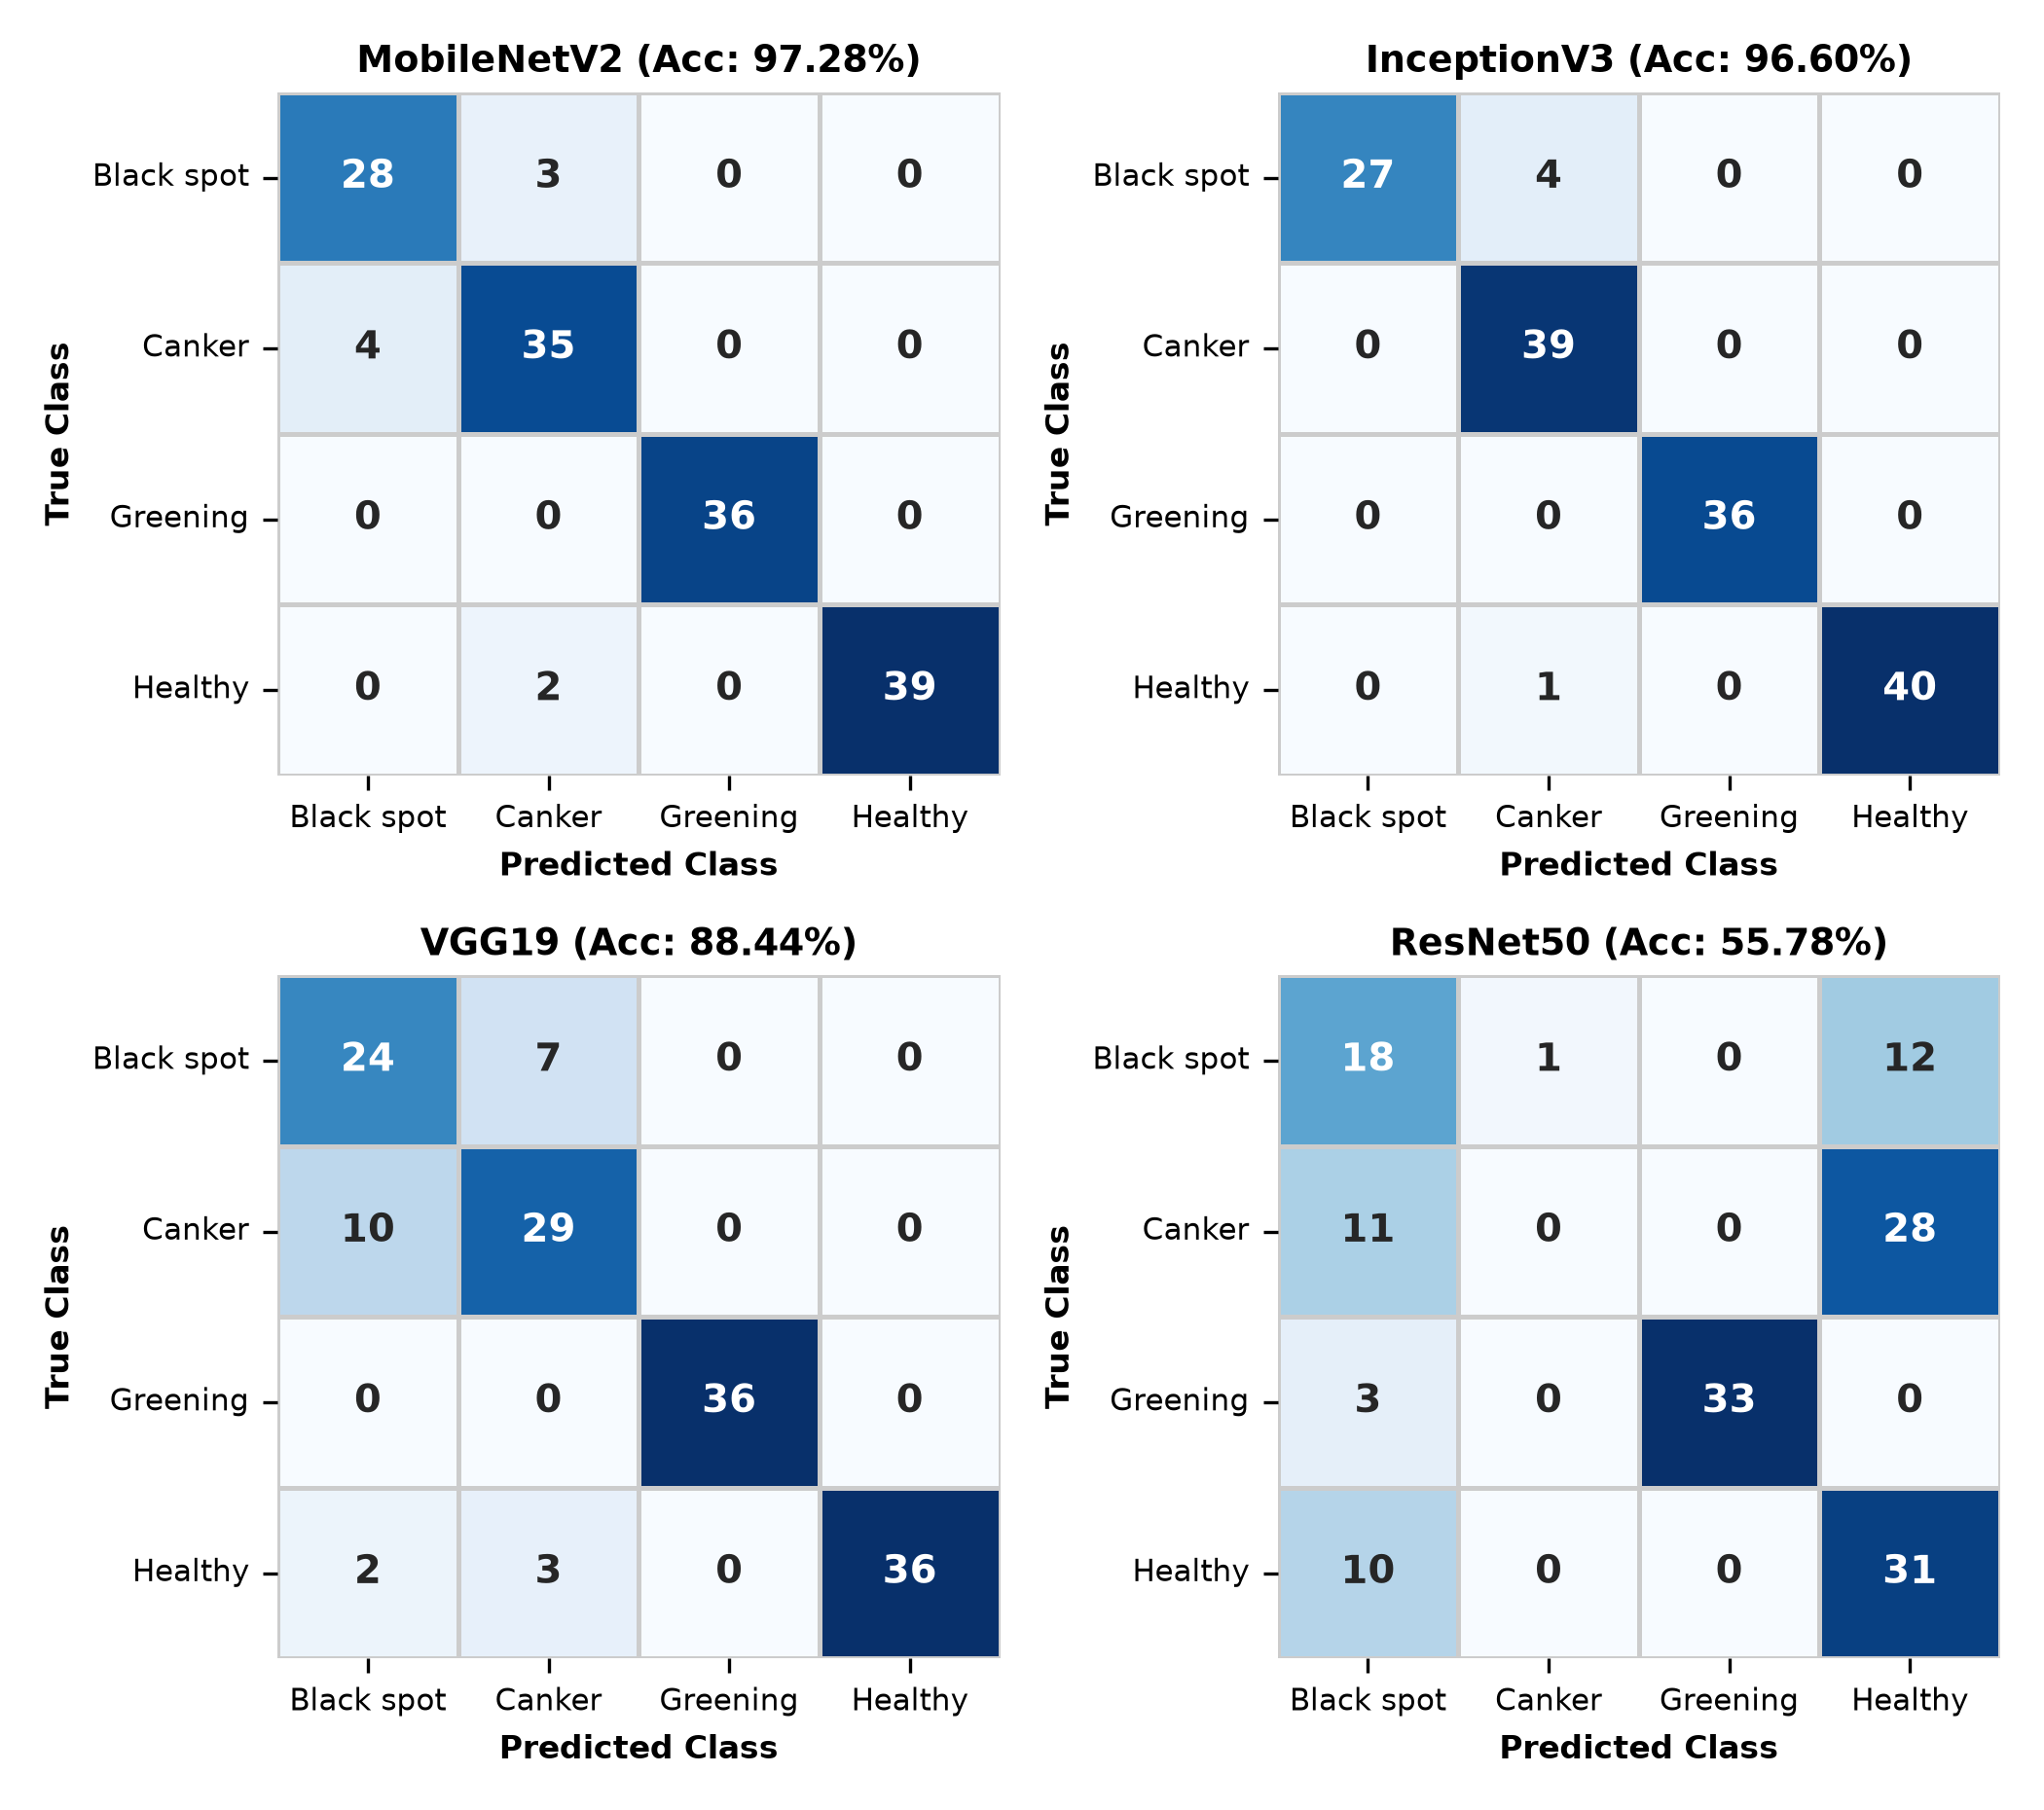
\includegraphics[width=0.88\columnwidth]{fig7_confusion_matrices.png}}
    \caption{Multi-class confusion matrices across all four fine-tuned CNN architectures on the test partition.}
    \label{fig:confusion matrix}
\end{figure}

\subsection{Computational Complexity Analysis}

For edge agricultural deployments, processing speed and memory demands are as critical as classification accuracy. Table~\ref{tab:complexity_metrics} compares training duration, test inference latency, and memory footprint across the models.

\begin{table}[htbp]
\tabcolsep4pt
\tbl{Quantitative Computational Complexity Metrics Across Models}{
\begin{tabular}{|l|c|c|c|c|}
\hline
\textbf{Metric} & \textbf{MobileNetV2} & \textbf{InceptionV3} &
\textbf{ResNet50} & \textbf{VGG19} \\
\hline
Training Time (s) & 406.29 & 717.00 & 1040.00 & 3360.14 \\
Inference Latency (s) & 83.67 & 85.73 & 84.11 & 80.34 \\
Memory Footprint (MB) & 9.82 & 22.81 & 34.28 & 118.59 \\
\hline
\end{tabular}}
\label{tab:complexity_metrics}
\end{table}

MobileNetV2 recorded the lowest training time (406.29~s) and the smallest memory footprint (9.82~MB). Compared to VGG19 (3360.14~s, 118.59~MB), MobileNetV2 reduced training time by 88\% and memory usage by 91.7\%. Inference times across all models were close, ranging between 80.34~s and 85.73~s for the 147 test images. Figure~\ref{fig:performance metrics} presents a graphical comparison of the performance metrics.

\begin{figure}[t]
    \centerline{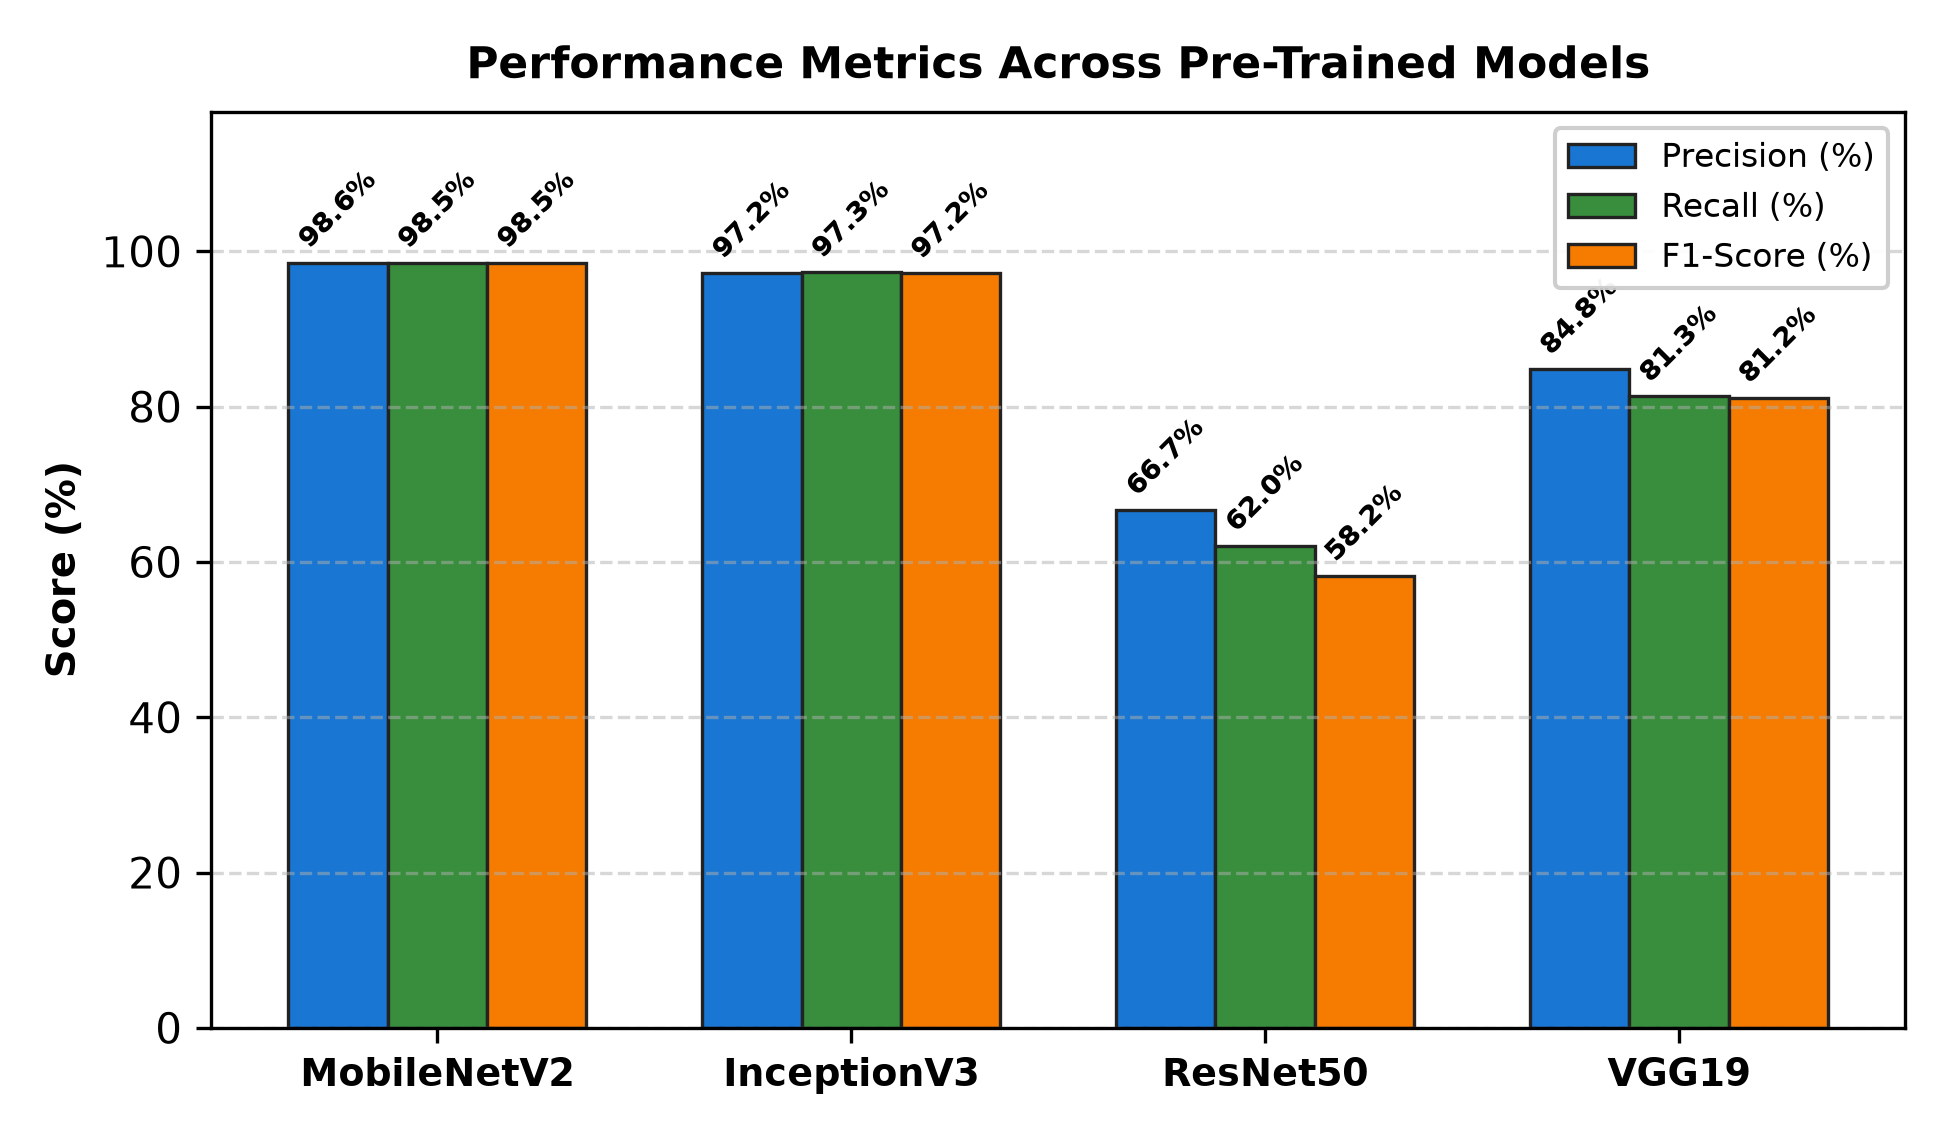
\includegraphics[width=0.88\columnwidth]{fig8_performance_metrics.png}}
    \caption{Comparative diagnostic metrics across the four pre-trained architectures.}
    \label{fig:performance metrics}
\end{figure}

\subsection{Comparative Discussion and Deployment Feasibility}

The experimental data shows that MobileNetV2 delivers the most effective balance of high accuracy and low resource usage. The inverted residual structure extracts rich visual features with few parameters. InceptionV3 reached similar accuracy, but required more memory (22.81~MB) and longer training (717.00~s). ResNet50 struggled under fixed-feature extraction, and VGG19 had high computational and memory costs.

These findings indicate that MobileNetV2 is the most practical option for deployment in field conditions, such as smartphone applications, portable scanning tools, and drone-mounted cameras for real-time orchard monitoring.

\section{Conclusion}
\label{sec:conclusion}

This study benchmarked four pre-trained deep learning models for multi-class citrus fruit disease diagnosis. Evaluating MobileNetV2, InceptionV3, ResNet50, and VGG19 on a 1,463-image dataset demonstrated that MobileNetV2 achieved superior overall performance: 96.77\% accuracy, 98.54\% F1-score, a 406.29~s training time, and a 9.82~MB memory footprint. These findings show that lightweight convolutional architectures can deliver high diagnostic accuracy while meeting edge device computational limits.

\subsection{Limitations}
The primary limitation of this work is the dataset size (1,463 images) and single-source acquisition environment. Field orchards often present variable lighting, partial occlusions, and overlapping leaf symptoms that require testing on larger multi-source datasets.

\subsection{Future Scope}
Future work will focus on:
\begin{itemize}
    \item Testing nature-inspired optimization algorithms (such as Grey Wolf Optimizer or Particle Swarm Optimization) for automated hyperparameter tuning.
    \item Developing lightweight hybrid vision transformers optimized for edge deployment.
    \item Integrating visual explanation methods, such as Grad-CAM, to highlight lesion regions for agricultural extension workers.
\end{itemize}

\bibliographystyle{ijcaArticle}
\bibliography{references}

\end{document}
